% Provenance (never printed): see sources/outline_sources.md (Year 1: continental
% rifting and break-up; passive-margin structure; fast and slow ridges; the depth--age
% law of the ocean floor; transform faults). Curve from figdata/bachelor-1/depth_age.py;
% exercise and problem values in the Book 3 scratch calculator calc/ch13.py; the
% coordinates of the margin schematic from calc/fig13_margin.py.
\chapter{Rifts, Ridges and Passive Margins}\label{ch:b1:rifts-ridges-margins}

In September 2005 the ground of the Afar desert, in the north-east of Ethiopia,
opened. Within three weeks a stretch of the rift some \qty{60}{km} long widened by up
to \qty{8}{m}, and about \qty{2.5}{km^3} of magma rose into the crack from
below. The plates there separate at about \qty{18}{mm} a year: the crisis
released, in a few weeks, the stretching of some four centuries. Afar is a
continent breaking apart; a few hundred kilometres to the north, the Red Sea
is a young ocean whose floor is already made like the floor of the Atlantic,
and the South Atlantic was such a rift before it opened, about 120 million
years ago. This chapter follows the birth of an ocean: the stretching of a
continent, its break-up, the two \omterm{def:b1:rifts-ridges-margins:passive-margin}{passive margins} left behind, the ridge that
builds the ocean floor, and the slow sinking of that floor as it cools.
% ledger: wright:afar, morvel:ar-nb (18.5 mm/yr at 12.3 N, 40.6 E, computed with euler_velocities.py), heine:fit

\begin{recall}
The plates are the upper \omterm{def:b1:heat-budget:boundary-layer}{thermal boundary layer} of the \omterm{def:b1:layered-earth:layers}{mantle}; under the
oceans a cooling half-space describes them, and their isotherms deepen as the
square root of age (\cref{ch:b1:heat-budget}). Columns of rock in isostatic
equilibrium have the same mass per unit area above a \omterm{def:b1:isostasy-gravity:isostasy}{compensation depth}
(\cref{ch:b1:isostasy-gravity}). Plates turn about \omterm{def:b1:plate-kinematics:euler-pole}{Euler poles}, ridges spread
at rates read from magnetic anomalies, and transforms lie on \omterm{def:b1:spherical-astronomy:spherical-triangle}{small circles}
about the pole (\cref{ch:b1:plate-kinematics}). The \omterm{def:b1:cross-sections:throw}{throw} and the \omterm{def:b1:cross-sections:throw}{heave} of a
fault were defined in \cref{ch:b1:cross-sections}; a normal fault is an
inclined fault whose upper block has moved down (Book 2, grade 11).
\end{recall}

\section{Continental rifting}

A continent stretched by forces at its edges does not thin evenly. Its brittle
upper \omterm{def:b1:layered-earth:layers}{crust} breaks along normal faults, and the blocks between them sink and
tilt; below, the warmer lower \omterm{def:b1:layered-earth:layers}{crust} and the \omterm{def:b1:layered-earth:layers}{mantle} flow.

\begin{definition}[Continental rift, graben, half-graben]\label{def:b1:rifts-ridges-margins:rift}
A \emph{continental rift}\index{continental rift} is a long, narrow zone where
a continent is being stretched: a depression bounded by normal faults, with
earthquakes and, often, volcanoes. A \emph{graben}\index{graben} is a block
dropped between two normal faults that \omterm{def:b1:geological-maps:attitude}{dip} towards each other. A
\emph{half-graben}\index{half-graben} is a block dropped and tilted against a
single major normal fault, the border fault, on one side only.
\end{definition}

Most rift basins are chains of \omterm{def:b1:rifts-ridges-margins:rift}{half-grabens}. Their border faults hand the
displacement over to one another through relay ramps, and the side of the
border fault often alternates from one segment to the next. The hanging wall
of each border fault tilts down towards it, and the basin fills fastest there:
the thickest sediment piles up against the fault, while the footwall is raised
into the rift shoulder.

The horizontal stretching carried by a fault is its \omterm{def:b1:cross-sections:throw}{heave}. A planar normal
fault of \omterm{def:b1:cross-sections:throw}{throw} $h$ and \omterm{def:b1:geological-maps:attitude}{dip} $\delta$ has the \omterm{def:b1:cross-sections:throw}{heave} $h/\tan\delta$
(\cref{ch:b1:cross-sections}); adding the \omterm{def:b1:cross-sections:throw}{heaves} of the faults across a rift
section gives the extension of the brittle \omterm{def:b1:layered-earth:layers}{crust}. How the whole \omterm{def:b1:layered-earth:lithosphere}{lithosphere}
thins as it is stretched, and why it then subsides, is quantified in the Year 2
volume; here the faults are measured, and their sum compared with the motion
of the plates.

\begin{omfigure}
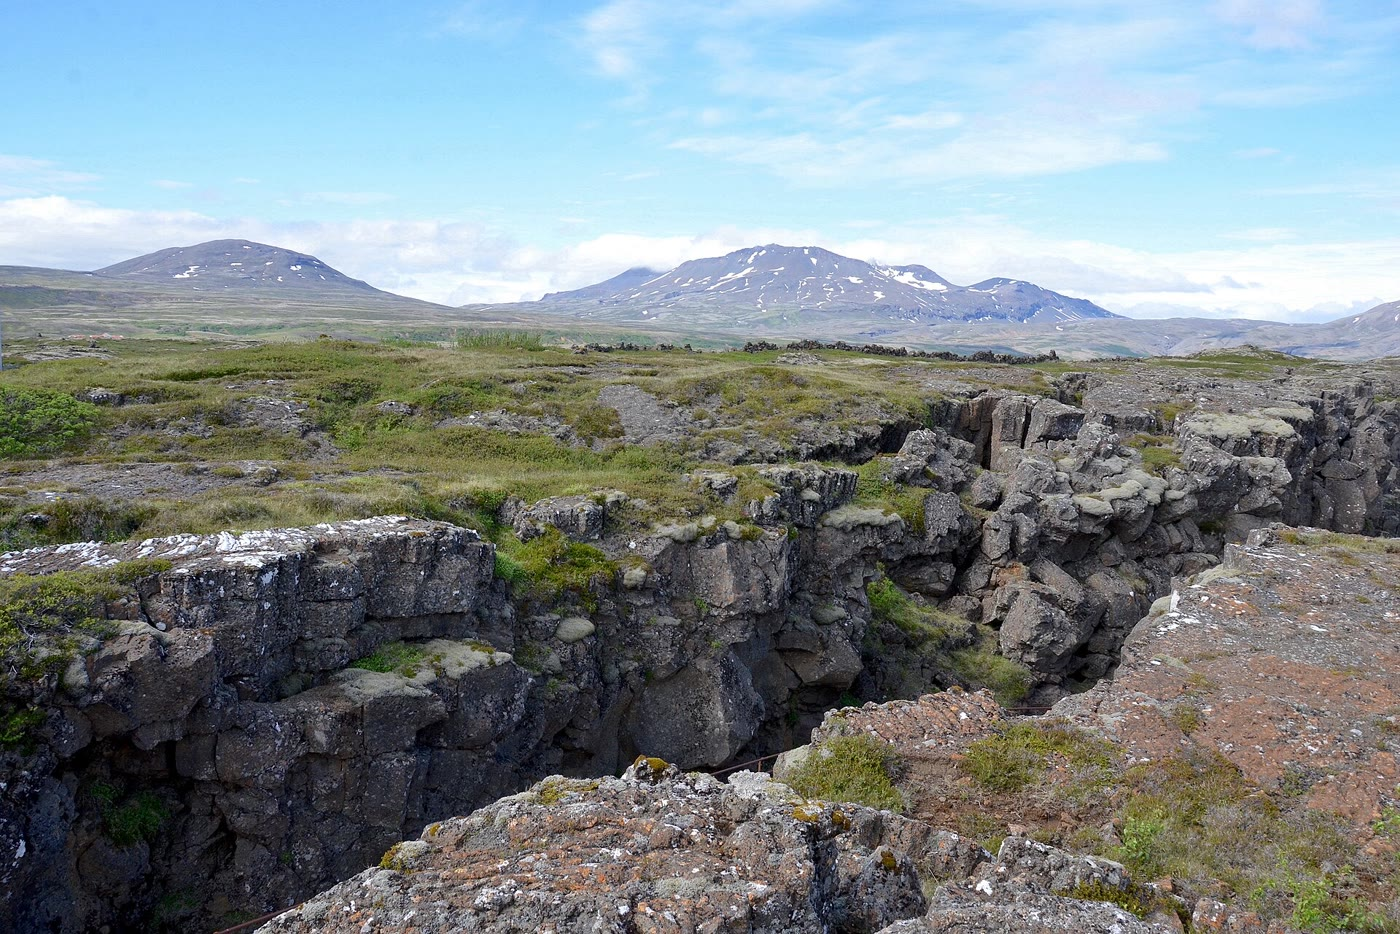
\includegraphics[width=0.8\linewidth]{images/book3/b1-thingvellir-fissure.jpg}

\par\smallskip{\small An open fissure in the lava floor of the Þingvellir rift
valley, in south-west Iceland, where the Mid-Atlantic Ridge comes ashore.
The basalt flows of the valley floor are cut by open fissures parallel to the
rift. Photograph: Olga Ernst,
CC~BY-SA~4.0 (Wikimedia Commons).}
\label{fig:b1:rifts-ridges-margins:thingvellir}
\end{omfigure}
% ledger: commons:thingvellir

\subsection*{Volcanic and magma-poor rifts}

Rifts differ in how much magma they receive. In a \emph{magma-poor} rift the
stretching is taken up by faults, and the \omterm{def:b1:layered-earth:layers}{crust} thins as the blocks slide
apart. In a volcanic rift magma takes over: dykes intrude the \omterm{def:b1:layered-earth:layers}{crust} along the
axis, each one opening the rift by its own thickness, and lavas flood the
surface. The East African Rift shows both, side by side: its eastern branch
is strongly volcanic, while its western branch is less so and holds deep
sedimentary basins, filled by lakes such as Lake Tanganyika and bounded by
faults.
% ledger: roberts:ear

Both branches began to form about 25 million years ago, and the rift splits
the African plate into a Nubian plate to the west and a Somali plate to the
east. From the Afar \omterm{def:b1:plate-kinematics:triple-junction}{triple junction} it runs south, in two branches around the
old, thick and cold Tanzania craton. Its motion is slow: computed
from the plate vectors of Somalia and Nubia, each measured relative to the
Antarctic plate, Somalia moves away from Nubia at \qty{6.0}{mm.yr^{-1}}
towards \ang{105} in central Ethiopia (\ang{8.5}\,N, \ang{39.5}\,E), and at
\qty{5.1}{mm.yr^{-1}} on the equator. Many earthquakes of the rift show
normal faulting.
% ledger: roberts:ear, morvel:sm-an, morvel:nb-an (SM-NB from SM-AN minus NB-AN, computed with figdata/bachelor-1/euler_velocities.py)

In Afar, at the northern end, the rift meets the Red Sea and the Gulf of Aden.
The bulk of the Ethiopian flood basalts erupted there about 30 million years
ago, in a million years or less, and magma has kept arriving since: lava flows
at the surface, intrusions in the \omterm{def:b1:layered-earth:layers}{crust} and new material added below it, so
much that the intruded \omterm{def:b1:layered-earth:layers}{crust} has kept its thickness through the early stages
of rifting. The crisis of 2005 shows how such a rift opens: not steadily, but
in episodes, each a dyke metres wide intruded within days or weeks. Since the
plates diverge at about \qty{18}{mm.yr^{-1}} there, the \qty{8}{m} dyke of
2005 took up the stretching of about 440 years.
% ledger: hofmann:traps, bastow:afar, wright:afar, morvel:ar-nb (rate computed with euler_velocities.py)

\section{Break-up and passive margins}

If stretching goes on, the continental \omterm{def:b1:layered-earth:layers}{crust} is thinned to nothing, the \omterm{def:b1:layered-earth:layers}{mantle}
rises beneath the rift and melts as it rises, and the first \omterm{def:b1:rifts-ridges-margins:oceanic-crust}{oceanic crust}
forms between the two halves of the continent. That moment is the
\emph{break-up}. From then on the plates move apart at a ridge in the middle of
a new ocean, and the two edges of the continent, carried away from the ridge,
stop being plate boundaries.

\begin{definition}[Passive margin, ocean--continent transition, break-up unconformity]\label{def:b1:rifts-ridges-margins:passive-margin}
A \emph{passive margin}\index{passive margin} is the edge of a continent that
was formed by rifting and is no longer a plate boundary: the continent and the
adjacent ocean floor belong to the same plate. The
\emph{ocean--continent transition}\index{ocean--continent transition} is the
zone of the margin, kilometres to tens of kilometres wide, between thinned
continental \omterm{def:b1:layered-earth:layers}{crust} and normal \omterm{def:b1:rifts-ridges-margins:oceanic-crust}{oceanic crust}. The \emph{break-up
unconformity}\index{break-up unconformity} is the \omterm{def:b1:cross-sections:unconformity}{unconformity} that separates
the sediments deposited in the rift basins, tilted with their blocks, from the
undisturbed sediments laid over the margin after break-up.
\end{definition}

\omterm{def:b1:rifts-ridges-margins:passive-margin}{Passive margins} line most of the Atlantic, the Arctic Ocean and the western Indian
Ocean, and nearly all the coasts of Africa, Australia, Greenland and India. The
eastern margin of North America and the north-western margin of Africa were
the two sides of one rift: they are \emph{conjugate} margins. Their profile is
the familiar sequence of the ocean floor near land: continental shelf, slope,
rise and abyssal plain. Under the shelf and slope lies the thinned continental
\omterm{def:b1:layered-earth:layers}{crust}, cut by normal faults that \omterm{def:b1:geological-maps:attitude}{dip} towards the ocean, with its rotated
blocks buried beneath the sediments.

\begin{omfigure}
\begin{tikzpicture}[x=0.95cm, y=0.9cm, font=\scriptsize]
% (a) continental rift: half-grabens on east-dipping faults; coordinates from calc/fig13_margin.py
\begin{scope}
\fill[green!25!gray!45] (0,-2) -- (3,-2) -- (6,-1.75) -- (9,-2) -- (12,-2) -- (12,-2.5) -- (0,-2.5) -- cycle;
\fill[orange!22] (0,0) -- (3.5,0) -- (3.931,-0.8) -- (4.75,-0.25) -- (5.05,-0.7) -- (6,-0.2) -- (6.223,-0.55) -- (7.25,-0.15) -- (7.402,-0.4) -- (8.6,0) -- (12,0) -- (12,-2) -- (9,-2) -- (6,-1.75) -- (3,-2) -- (0,-2) -- cycle;
\fill[yellow!45] (3.565,-0.12) -- (3.931,-0.8) -- (4.75,-0.25) -- (4.75,-0.12) -- cycle;
\fill[yellow!45] (4.75,-0.12) -- (4.75,-0.25) -- (5.05,-0.7) -- (6,-0.2) -- (6,-0.12) -- cycle;
\fill[yellow!45] (6,-0.12) -- (6,-0.2) -- (6.223,-0.55) -- (7.25,-0.15) -- (7.25,-0.12) -- cycle;
\fill[yellow!45] (7.25,-0.12) -- (7.25,-0.15) -- (7.402,-0.4) -- (8.241,-0.12) -- cycle;
\draw (0,0) -- (3.5,0) -- (3.931,-0.8) -- (4.75,-0.25) -- (5.05,-0.7) -- (6,-0.2) -- (6.223,-0.55) -- (7.25,-0.15) -- (7.402,-0.4) -- (8.6,0) -- (12,0);
\draw[contact] (0,-2) -- (3,-2) -- (6,-1.75) -- (9,-2) -- (12,-2);
\draw[fault] (3.5,0) -- (4.2,-1.3);
\draw[fault] (4.75,-0.25) -- (5.45,-1.3);
\draw[fault] (6,-0.2) -- (6.7,-1.3);
\draw[fault] (7.25,-0.15) -- (7.95,-1.3);
\node[anchor=west, font=\small\bfseries] at (0,0.75) {(a) continental rift};
\node[anchor=south] at (2.2,0) {rift shoulder};
\node[anchor=south, align=center] at (6.3,0) {half-grabens filled with sediment};
\draw[-{Stealth[length=3pt]}] (2.6,-0.75) node[anchor=east] {border fault} -- (3.75,-0.5);
\node at (9.8,-1.0) {continental crust};
\node at (10.3,-2.25) {mantle};
\node at (6,-2.18) {Moho raised under the rift};
\end{scope}
% (b) break-up: conjugate halves, the first oceanic crust between them
\begin{scope}[yshift=-3.6cm]
\fill[omSea!35] (2.8,0) -- (9.2,0) -- (9.2,-1.3) -- (2.8,-1.3) -- cycle;
\fill[green!25!gray!45] (0,-2) -- (2.5,-2) -- (5.5,-1.3) -- (6.5,-1.3) -- (9.5,-2) -- (12,-2) -- (12,-2.5) -- (0,-2.5) -- cycle;
\fill[orange!22] (0,0) -- (2.8,0) -- (3.146,-0.75) -- (3.8,-0.3) -- (4.13,-0.85) -- (4.7,-0.45) -- (5.053,-0.95) -- (5.5,-1) -- (5.5,-1.3) -- (2.5,-2) -- (0,-2) -- cycle;
\fill[orange!22] (12,0) -- (9.2,0) -- (8.854,-0.75) -- (8.2,-0.3) -- (7.87,-0.85) -- (7.3,-0.45) -- (6.947,-0.95) -- (6.5,-1) -- (6.5,-1.3) -- (9.5,-2) -- (12,-2) -- cycle;
\fill[lith basalt] (5.5,-1) -- (6.5,-1) -- (6.5,-1.3) -- (5.5,-1.3) -- cycle;
\draw (0,0) -- (2.8,0) -- (3.146,-0.75) -- (3.8,-0.3) -- (4.13,-0.85) -- (4.7,-0.45) -- (5.053,-0.95) -- (5.5,-1) -- (6.5,-1) -- (6.947,-0.95) -- (7.3,-0.45) -- (7.87,-0.85) -- (8.2,-0.3) -- (8.854,-0.75) -- (9.2,0) -- (12,0);
\draw[contact] (0,-2) -- (2.5,-2) -- (5.5,-1.3) -- (6.5,-1.3) -- (9.5,-2) -- (12,-2);
\draw[omSea!70!black] (2.8,0) -- (9.2,0);
\draw[fault] (2.8,0) -- (3.4,-1.3);
\draw[fault] (3.8,-0.3) -- (4.4,-1.3);
\draw[fault] (4.7,-0.45) -- (5.3,-1.3);
\draw[fault] (9.2,0) -- (8.6,-1.3);
\draw[fault] (8.2,-0.3) -- (7.6,-1.3);
\draw[fault] (7.3,-0.45) -- (6.7,-1.3);
\draw[omRidge, very thick, -{Stealth[length=3pt]}] (6,-2.3) -- (6,-1.45);
\node[anchor=west, font=\small\bfseries] at (0,0.75) {(b) break-up};
\node[anchor=south] at (6,0) {the sea floods the rift};
\node[anchor=west] at (6.15,-2.1) {mantle rises and melts};
\node[anchor=south, fill=white, fill opacity=0.8, text opacity=1, inner sep=1pt, align=center] at (6,-0.85) {first oceanic\\crust};
\node at (1.4,-1.0) {tilted blocks};
\node at (10.6,-1.0) {tilted blocks};
\node at (1.4,-2.25) {mantle};
\end{scope}
% (c) one passive margin after drift
\begin{scope}[yshift=-7.4cm]
\fill[omSea!35] (1.2,0.3) -- (12,0.3) -- (12,-1.2) -- (8.2,-1.15) -- (6.4,-0.9) -- (4.6,0.1) -- cycle;
\fill[green!25!gray!45] (0,-2.3) -- (2,-2.3) -- (5.9,-1.8) -- (6.7,-2.1) -- (12,-2.1) -- (12,-2.7) -- (0,-2.7) -- cycle;
\fill[orange!22] (0,0.3) -- (1.2,0.3) -- (2.2,0) -- (3,-0.25) -- (3.259,-0.95) -- (4,-0.55) -- (4.286,-1.15) -- (4.9,-0.85) -- (5.233,-1.35) -- (5.9,-1.55) -- (5.9,-1.8) -- (2,-2.3) -- (0,-2.3) -- cycle;
\fill[pattern=crosshatch dots, pattern color=green!40!black] (5.9,-1.55) -- (6.4,-1.75) -- (6.7,-2.1) -- (5.9,-1.8) -- cycle;
\fill[lith basalt] (6.4,-1.75) -- (12,-1.75) -- (12,-2.1) -- (6.7,-2.1) -- cycle;
\fill[yellow!45] (3,-0.25) -- (3.259,-0.95) -- (4,-0.55) -- cycle;
\fill[yellow!45] (4,-0.55) -- (4.286,-1.15) -- (4.9,-0.85) -- cycle;
\fill[yellow!45] (4.9,-0.85) -- (5.233,-1.35) -- (5.9,-1.55) -- (5.9,-1.45) -- cycle;
\fill[yellow!15] (1.2,0.3) -- (4.6,0.1) -- (6.4,-0.9) -- (8.2,-1.15) -- (12,-1.2) -- (12,-1.75) -- (6.4,-1.75) -- (5.9,-1.55) -- (5.9,-1.45) -- (4.9,-0.85) -- (4,-0.55) -- (3,-0.25) -- (2.2,0) -- cycle;
\draw[black!45] (2.4,0.12) -- (4.8,-0.1) -- (6.6,-1.05) -- (8.4,-1.27) -- (12,-1.31);
\draw (1.2,0.3) -- (4.6,0.1) -- (6.4,-0.9) -- (8.2,-1.15) -- (12,-1.2);
\draw[omSea!70!black] (1.2,0.3) -- (12,0.3);
\draw[unconformity] (2.2,0) -- (3,-0.25) -- (4,-0.55) -- (4.9,-0.85) -- (5.9,-1.45);
\draw (3.259,-0.95) -- (4,-0.55) (4.286,-1.15) -- (4.9,-0.85) (5.233,-1.35) -- (5.9,-1.55) -- (6.4,-1.75) -- (12,-1.75);
\draw[contact] (0,-2.3) -- (2,-2.3) -- (5.9,-1.8) -- (6.7,-2.1) -- (12,-2.1);
\draw[fault] (3,-0.25) -- (3.5,-1.6);
\draw[fault] (4,-0.55) -- (4.5,-1.6);
\draw[fault] (4.9,-0.85) -- (5.4,-1.6);
\node[anchor=west, font=\small\bfseries] at (0,0.95) {(c) passive margin};
\node[anchor=south] at (3.4,0.25) {shelf};
\node[anchor=south west] at (5.6,-0.45) {slope};
\node[anchor=south] at (8.4,-1.12) {rise};
\node[anchor=south] at (10.6,-1.17) {abyssal plain};
\node[anchor=south] at (10.6,-0.1) {ocean};
\node at (9.8,-1.53) {post-rift sediments};
\node[fill=white, fill opacity=0.8, text opacity=1, inner sep=1pt, align=center] (bu) at (1.0,-0.6) {break-up\\unconformity};
\draw[-{Stealth[length=3pt]}] (bu.east) -- (2.55,-0.16);
\node[fill=white, fill opacity=0.8, text opacity=1, inner sep=1pt, align=center] (sr) at (1.6,-1.35) {syn-rift\\sediments};
\draw[-{Stealth[length=3pt]}] (sr.east) -- (3.45,-0.75);
\node at (1.3,-1.98) {continental crust};
\draw[decorate, decoration={brace, amplitude=3pt, mirror}] (5.9,-2.17) -- (6.7,-2.17) node[midway, below=3pt, align=center] {ocean--continent\\transition};
\node[anchor=west, fill=white, fill opacity=0.85, text opacity=1, inner sep=1pt] at (8.6,-1.93) {oceanic crust};
\node at (3.6,-2.5) {mantle};
\end{scope}
\end{tikzpicture}

\par\smallskip{\small From rift to \omterm{def:b1:rifts-ridges-margins:passive-margin}{passive margin} (drawings, not to scale; the
heights are exaggerated). (a) The brittle upper \omterm{def:b1:layered-earth:layers}{crust} breaks along normal
faults; blocks tilt into \omterm{def:b1:rifts-ridges-margins:rift}{half-grabens} that fill with sediment, and the \omterm{def:b1:layered-earth:discontinuity}{Moho}
rises under the thinned \omterm{def:b1:layered-earth:layers}{crust}. (b) At break-up the continental \omterm{def:b1:layered-earth:layers}{crust} is cut
through; the sea floods the rift and the first \omterm{def:b1:rifts-ridges-margins:oceanic-crust}{oceanic crust} forms. (c) One
of the two margins, carried away from the ridge: its tilted blocks and their
sediments lie under the \omterm{def:b1:rifts-ridges-margins:passive-margin}{break-up unconformity}, buried by the post-rift
sediments of the shelf, slope and rise.}
\label{fig:b1:rifts-ridges-margins:margin}
\end{omfigure}

\subsection*{Two kinds of margin}

Margins inherit the character of their rift. On \emph{magma-poor} margins,
such as those of Iberia and Newfoundland, the seismic sections show rotated
blocks whose beds \omterm{def:b1:geological-maps:attitude}{dip} towards the continent; in places the \omterm{def:b1:rifts-ridges-margins:passive-margin}{ocean--continent
transition} is floored by \omterm{def:b1:layered-earth:layers}{mantle} peridotite, brought up to the sea floor and
altered by sea water to serpentinite. On \emph{volcanic} margins, such as the
mid-Norwegian, East Greenland, Namibian and Brazilian margins, the transition
is built of basalt: stacks of lava flows that \omterm{def:b1:geological-maps:attitude}{dip} towards the ocean, the
seaward-dipping reflectors of seismic sections, and below them a lower \omterm{def:b1:layered-earth:layers}{crust}
in which P waves travel unusually fast, magma added beneath the \omterm{def:b1:layered-earth:layers}{crust} at
break-up. Volcanic margins subside little during break-up.

\begin{inthefield}[Finding the edge of a continent]
The \omterm{def:b1:rifts-ridges-margins:passive-margin}{ocean--continent transition} lies under kilometres of water and sediment,
and is located only by geophysics, usually by several methods together.
Seismic reflection images the tilted blocks, the \omterm{def:b1:rifts-ridges-margins:passive-margin}{break-up unconformity} and,
where the signal reaches deep enough, the \omterm{def:b1:layered-earth:discontinuity}{Moho}. Wide-angle seismic refraction
measures the speeds of P waves through the \omterm{def:b1:layered-earth:layers}{crust}, which differ between
continental and \omterm{def:b1:rifts-ridges-margins:oceanic-crust}{oceanic crust}. Gravity data, inverted for the depth of the
\omterm{def:b1:layered-earth:discontinuity}{Moho}, give the thickness of the \omterm{def:b1:layered-earth:layers}{crust}. The magnetic stripes of the ocean floor
stop where the continental \omterm{def:b1:layered-earth:layers}{crust}, magnetically quiet, begins.
\end{inthefield}

After break-up a margin sinks. During rifting the \omterm{def:b1:layered-earth:lithosphere}{lithosphere} was thinned and
heated; carried away from the ridge, it cools and contracts, like the ocean
floor beside it, and the space that opens above it fills with the wedge of
post-rift sediments, whose weight presses it down further. The cooling half of
this story is told in \cref{sec:b1:rifts-ridges-margins:depth-age}; the
weight of the sediments is the subject of \cref{ch:b1:diagenesis-basins}.

\section{Fast and slow ridges}

Once the ocean is born, it grows at its ridge. Ridges spread at very different
rates: the rates measured over the last few million years run from
\qty{9.7}{mm.yr^{-1}} in the northern Red Sea to \qty{154.4}{mm.yr^{-1}} on
the East Pacific Rise. Their shape depends on that rate.
% ledger: morvel:range

\begin{definition}[Fast-, slow- and ultraslow-spreading ridges]\label{def:b1:rifts-ridges-margins:ridge-classes}
A ridge is classed by its \omterm{def:b1:plate-kinematics:spreading-rate}{full spreading rate}. An
\emph{ultraslow-spreading ridge}\index{ultraslow-spreading ridge} opens at
less than about \qty{20}{mm.yr^{-1}}; a \emph{slow-spreading
ridge}\index{slow-spreading ridge} at 20 to \qty{55}{mm.yr^{-1}}; an
intermediate ridge at 55 to \qty{75}{mm.yr^{-1}}; a \emph{fast-spreading
ridge}\index{fast-spreading ridge} at more than about
\qty{75}{mm.yr^{-1}}.
\end{definition}
% ledger: seton:rate-classes, dick:ultraslow

The limits are conventions and vary between authors. What does not vary is the
change of form. A slow ridge, such as the Mid-Atlantic Ridge, has
an axial valley between inward-facing normal faults: the gap between the
plates is not filled by magma as fast as it opens, and the cold \omterm{def:b1:layered-earth:lithosphere}{lithosphere}
breaks. A fast ridge, such as the East Pacific Rise, has no rift valley but a
smooth axial high over a lens of melt, refilled often enough to keep pace.
Either way the axis lies about \qty{2500}{m} deep, and the oldest floor of the
basins nearly \qty{4}{km} deeper (\cref{sec:b1:rifts-ridges-margins:depth-age}).
% ledger: parsons:plate-model (6400 - 2500 m)

Ultraslow ridges show what happens when magma is scarcest: their volcanism is
intermittent, they lack \omterm{def:b1:rifts-ridges-margins:transform}{transform faults}, and over large regions the \omterm{def:b1:layered-earth:layers}{mantle}
itself is brought up to the sea floor. The Gakkel Ridge, under the Arctic
Ocean, the slowest of all, is not offset at all; along a central stretch of
its axis some \qty{300}{km} long, \omterm{def:b1:layered-earth:layers}{mantle} peridotite lies directly on the axis,
between abundant volcanism to the west and large, widely spaced volcanoes to
the east. On slow and ultraslow ridges especially, part of the spreading is
taken up by long, gently dipping normal faults, detachments, whose footwall is
pulled out from under the axis: gabbro and peridotite reach the sea floor in
corrugated domes, \emph{oceanic core complexes}. The Atlantis Massif, beside
the Mid-Atlantic Ridge near \ang{30}\,N, is one: on its top, on \omterm{def:b1:layered-earth:layers}{crust}
\qty{1.5}{Myr} old about \qty{15}{km} from the axis, sea water reacting with
the \omterm{def:b1:layered-earth:layers}{mantle} rock feeds the warm, alkaline springs of the Lost City
hydrothermal field.
% ledger: dick:ultraslow, michael:gakkel, kelley:lost-city

\subsection*{The oceanic crust}

\begin{definition}[Oceanic crust, pillow lava, sheeted dyke complex]\label{def:b1:rifts-ridges-margins:oceanic-crust}
The \emph{oceanic crust}\index{oceanic crust} is the \omterm{def:b1:layered-earth:layers}{crust} made at ocean
ridges: 6 to \qty{7}{km} of basalt and gabbro, from the sea floor down to the
\omterm{def:b1:layered-earth:discontinuity}{Moho}, beneath a cover of sediments. \emph{Pillow lava}\index{pillow lava} is
lava erupted under water, made of rounded, interconnected tubes and lobes, each
with a glassy skin chilled by the sea. A \emph{sheeted dyke
complex}\index{sheeted dyke complex} is a layer made almost entirely of
parallel vertical dykes, each intruded into the previous ones.
\end{definition}

The layers of the \omterm{def:b1:rifts-ridges-margins:oceanic-crust}{oceanic crust} were first defined by seismology, then sampled
by drilling and recognised in slices of ocean floor thrust onto continents,
the ophiolites. From the top:
\begin{itemize}
  \item layer~1, sediments, thin or absent near the ridge and thickening with
        the age of the floor;
  \item layer~2, on average \qty{1.84}{km} of basalt: \omterm{def:b1:rifts-ridges-margins:oceanic-crust}{pillow lava} at the top
        (layer~2A), sheeted dykes of diabase below (layer~2B);
  \item layer~3, the remaining four to five kilometres, of gabbro and, at its
        base, cumulates settled from the magma: some \qty{70}{\percent} of
        the thickness of the \omterm{def:b1:layered-earth:layers}{crust}.
\end{itemize}
Beneath the \omterm{def:b1:layered-earth:discontinuity}{Moho} lies \omterm{def:b1:layered-earth:layers}{mantle} peridotite, the residue left by the melting.
% ledger: christeson:crust, white:crust (layer 3: 6.15 - 1.84 = 4.3 km, 70 %; 7.1 - 1.84 = 5.3 km)

Seismic refraction gives the igneous \omterm{def:b1:layered-earth:layers}{crust} a mean thickness of
\qty[uncertainty-mode=separate]{7.1 \pm 0.8}{km} away from \omterm{def:b1:rifts-ridges-margins:transform}{fracture zones} and
hot spots, and a later synthesis of seismic profiles \qty{6.15}{km}, much the
same at all spreading rates: the amount of melt depends on the temperature of
the rising \omterm{def:b1:layered-earth:layers}{mantle}, not on the speed at which it rises. Only very slow ridges
make anomalously thin \omterm{def:b1:layered-earth:layers}{crust}: the \omterm{def:b1:layered-earth:layers}{mantle} there has time to cool as it rises,
and melts less. Over a hot plume the \omterm{def:b1:layered-earth:layers}{crust} is thicker, about \qty{20}{km}
directly above the rising core of a plume, as under Iceland
(\cref{ch:b1:hotspots}). Along all the ridges together, about
\qty{3.0}{km^2} of new sea floor and some \qty{20}{km^3} of new \omterm{def:b1:layered-earth:layers}{crust} are made
each year.
% ledger: white:crust, christeson:crust, data:pb2002 (production summed over the spreading steps in figdata/bachelor-1/ridge_budget.py)

\begin{omfigure}
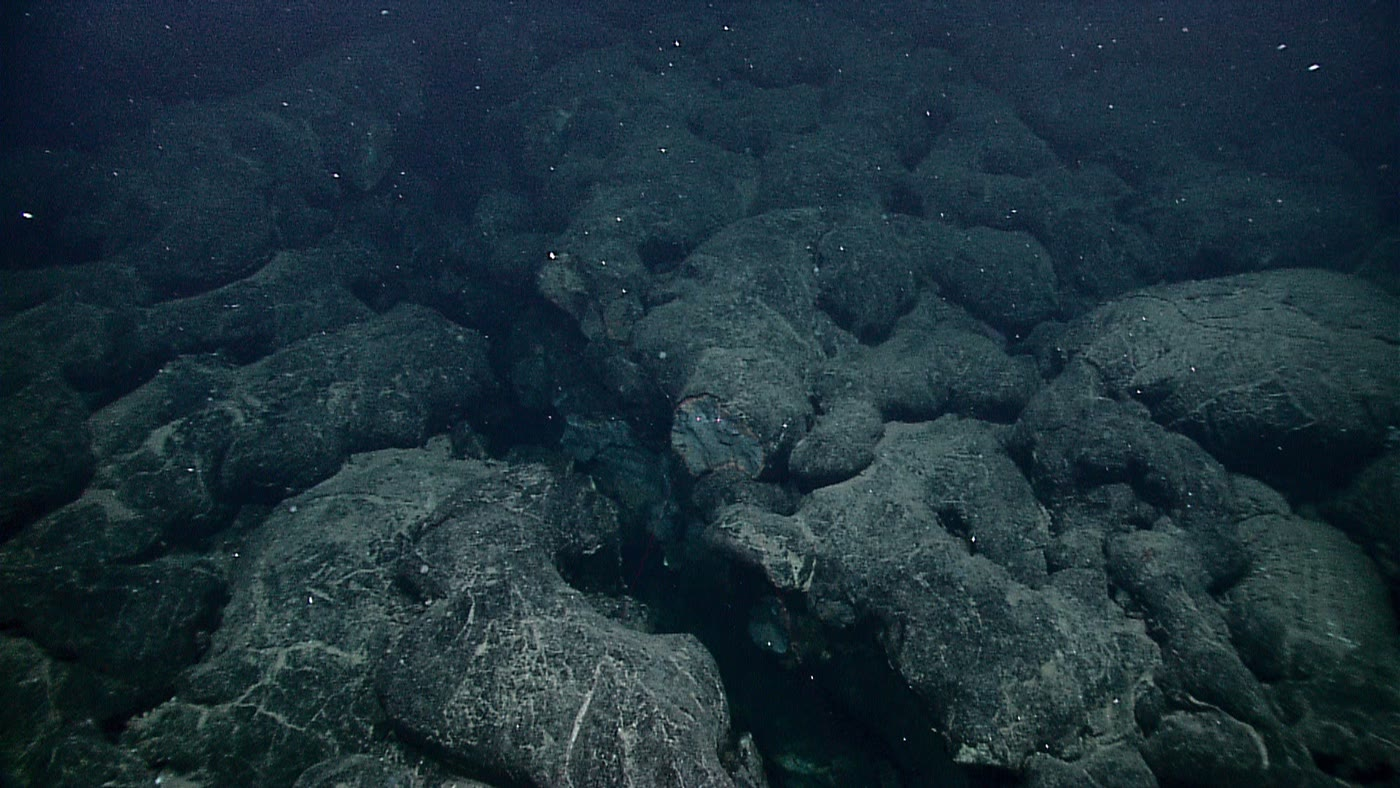
\includegraphics[width=0.6\linewidth]{images/book3/b1-pillow-lava.jpg}

\par\smallskip{\small \omterm{def:b1:rifts-ridges-margins:oceanic-crust}{Pillow lavas} on the Galápagos Rift, cut by a fissure
that opened after they had set: the top of layer~2 of the \omterm{def:b1:rifts-ridges-margins:oceanic-crust}{oceanic crust} as it
forms. Each pillow is a tongue of lava frozen from the outside by the sea
water. Photograph: NOAA Okeanos Explorer Program, Galápagos Rift Expedition
2011, CC~BY~2.0 (Wikimedia Commons).}
\label{fig:b1:rifts-ridges-margins:pillows}
\end{omfigure}
% ledger: commons:pillow-expl6453

\begin{proposition}[Each dyke splits the one before]\label{prop:b1:rifts-ridges-margins:dykes}
Suppose that every dyke of a \omterm{def:b1:rifts-ridges-margins:oceanic-crust}{sheeted dyke complex} is intruded along the axis
of spreading, where the \omterm{def:b1:layered-earth:layers}{crust} is hottest and weakest, and that the \omterm{def:b1:layered-earth:layers}{crust} moves
away from the axis symmetrically. Then most dykes are found split in two, each
half with a chilled margin against its older neighbour only.
\end{proposition}

\begin{proof}
A dyke chills against the colder rock on both sides: it has two chilled
margins when it forms. The next dyke rises where the \omterm{def:b1:layered-earth:layers}{crust} is weakest, along
the axis, that is, through the middle of the previous one, still the hottest
rock. It splits it into two halves, which the spreading carries away on either
side; each half keeps the chilled margin on its outer side and has, on its inner
side, the uncooled contact with the new dyke. Every dyke but the last is split
in this way.
\end{proof}

Dykes with a chilled margin on one side only are indeed the rule in \omterm{def:b1:rifts-ridges-margins:oceanic-crust}{sheeted
dyke complexes}: the signature of a \omterm{def:b1:layered-earth:layers}{crust} built, dyke after dyke, by
spreading.


\section{The depth--age law}\label{sec:b1:rifts-ridges-margins:depth-age}

Ocean floor is shallow at the ridge and deep far from it. Since floor is made
at the ridge and carried away, distance from the ridge is age, and the depth of
the floor depends on its age. The plate cools from above as it ages
(\cref{ch:b1:heat-budget}); cold rock is denser, and a denser column floats
lower.

\begin{lemma}[An integral of the error function]\label{lem:b1:rifts-ridges-margins:erfc}
With $\operatorname{erfc} u = 1 - \operatorname{erf} u =
\frac{2}{\sqrt\pi}\int_u^\infty e^{-s^2}\,\mathrm ds$,
\[
  \int_0^\infty \operatorname{erfc} u \,\mathrm du = \frac{1}{\sqrt\pi}.
\]
\end{lemma}

\begin{proof}
The derivative of $\operatorname{erfc}$ is $-\frac{2}{\sqrt\pi}e^{-u^2}$.
Integrating by parts on $[0, X]$,
\[
  \int_0^X \operatorname{erfc} u\,\mathrm du
  = \bigl[u \operatorname{erfc} u\bigr]_0^X + \frac{2}{\sqrt\pi}\int_0^X u\,e^{-u^2}\,\mathrm du
  = X\operatorname{erfc} X + \frac{1}{\sqrt\pi}\bigl(1 - e^{-X^2}\bigr).
\]
For $X > 0$ and $s \ge X$, $e^{-s^2} \le (s/X)e^{-s^2}$, so
$X\operatorname{erfc} X \le \frac{2}{\sqrt\pi}\int_X^\infty s\,e^{-s^2}\,\mathrm ds
= e^{-X^2}/\sqrt\pi$, which tends to 0. Letting $X \to \infty$ gives the
result.
\end{proof}

\begin{theorem}[Depth--age law]\label{thm:b1:rifts-ridges-margins:depth-age}
Suppose that
\begin{enumerate}
  \item the \omterm{def:b1:layered-earth:layers}{mantle} leaves the ridge at the uniform temperature $T_m$, and the
        oceanic plate of age $t$ is a half-space cooled since then from its
        surface, held at $T_0$, with the thermal diffusivity $\kappa$;
  \item the density of the cooled rock is $\rho_m\bigl(1 + \alpha(T_m -
        T)\bigr)$, with $\rho_m$ the density of the \omterm{def:b1:layered-earth:layers}{mantle} at $T_m$ and
        $\alpha$ its coefficient of thermal expansion;
  \item every column is in isostatic equilibrium above a \omterm{def:b1:isostasy-gravity:isostasy}{compensation depth}
        lying below the cooled layer, and sea water has the density $\rho_w$.
\end{enumerate}
Then the depth of the sea floor of age $t$ is
\[
  d(t) = d_r + C\sqrt t, \qquad
  C = \frac{2}{\sqrt\pi}\,\frac{\rho_m\,\alpha\,(T_m - T_0)\sqrt\kappa}{\rho_m - \rho_w},
\]
where $d_r$ is the depth of the ridge axis. This is the
\emph{depth--age law}\index{depth--age law} of the ocean floor.
\end{theorem}

\begin{proof}
The temperature in the cooled half-space is
\[
  T(z, t) = T_0 + (T_m - T_0)\operatorname{erf}\frac{z}{2\sqrt{\kappa t}},
\]
with $z$ the depth below the sea floor; this solution of the heat equation is
admitted here, as in \cref{ch:b1:heat-budget}, and derived in the Year 3
volume. Compare the column at the ridge, made of water down to $d_r$ and of
\omterm{def:b1:layered-earth:layers}{mantle} at $T_m$ below, with the column of age $t$, made of water down to $d$ and
of the cooled plate below, both down to the \omterm{def:b1:isostasy-gravity:isostasy}{compensation depth} $D$. Their masses
per unit area are equal:
\[
  \rho_w d_r + \rho_m (D - d_r) = \rho_w d + \int_0^{D-d}\rho_m\bigl(1 + \alpha(T_m - T)\bigr)\mathrm dz
  = \rho_w d + \rho_m (D - d) + \rho_m\alpha\int_0^{D-d}(T_m - T)\,\mathrm dz.
\]
Hence
\[
  (\rho_m - \rho_w)(d - d_r) = \rho_m\alpha\int_0^{D-d}(T_m - T)\,\mathrm dz.
\]
Since $T_m - T = (T_m - T_0)\operatorname{erfc}\bigl(z/2\sqrt{\kappa t}\bigr)$ is
negligible below the cooled layer, the integral may be taken to infinity; with
$u = z/2\sqrt{\kappa t}$ and \cref{lem:b1:rifts-ridges-margins:erfc},
\[
  \int_0^\infty (T_m - T)\,\mathrm dz = (T_m - T_0)\,2\sqrt{\kappa t}\int_0^\infty\operatorname{erfc}u\,\mathrm du
  = \frac{2}{\sqrt\pi}(T_m - T_0)\sqrt{\kappa t}.
\]
Dividing by $\rho_m - \rho_w$ gives $d - d_r = C\sqrt t$.
\end{proof}

The water matters: as the plate sinks, water fills the space above it, and its
weight presses the plate further down. The effective expansion coefficient
$\alpha\rho_m/(\rho_m - \rho_w)$ is larger than $\alpha$ by the factor
$3300/2300 \approx 1.43$.

With $\alpha = \qty{3.2e-5}{K^{-1}}$, $T_m - T_0 = \qty{1350}{K}$,
$\kappa = \qty{e-6}{m^2.s^{-1}}$, $\rho_m = \qty{3300}{kg.m^{-3}}$ and
$\rho_w = \qty{1000}{kg.m^{-3}}$, and time counted in millions of years
($\sqrt{\kappa\times\qty{1}{Myr}} = \qty{5618}{m}$), the theorem gives
$C = \qty{393}{m.Myr^{-1/2}}$. The constants fitted by Parsons and Sclater to
the depths of the North Pacific and the North Atlantic, once the sediments are
removed, are close: $d_r \approx \qty{2500}{m}$ and
$C \approx \qty{350}{m.Myr^{-1/2}}$, from 0 to \qty{70}{Myr}. The values of
$\alpha$ and $T_m$ used above are those of their plate model for old floor,
a \omterm{def:b1:layered-earth:layers}{mantle} at \qty{1350}{\degreeCelsius} and
$\alpha = \qty{3.2e-5}{\per\degreeCelsius}$, uncertain by a fifth and a third
respectively, so that the agreement of 393 with 350 is as good as could be
hoped.
% ledger: parsons:plate-model, ps77:depth-age

\begin{example}[Ocean floor 25 and 100 million years old]\label{ex:b1:rifts-ridges-margins:depths}
With $d = 2500 + 350\sqrt t$ (metres, $t$ in millions of years), floor
\qty{25}{Myr} old lies at $2500 + 350\times5 = \qty{4250}{m}$ and floor
\qty{100}{Myr} old at $2500 + 350\times10 = \qty{6000}{m}$. The floor sinks
\qty{1750}{m} in its first 25 million years, and only \qty{1750}{m} more in
the next 75.
\end{example}
% ledger: parsons:plate-model

\begin{omfigure}
\begin{tikzpicture}
\begin{axis}[omrecord, omdepth, width=0.84\linewidth, height=6.6cm,
  xmin=0, xmax=13.6, ymin=2000, ymax=6800,
  xlabel={square root of the age of the floor, $\sqrt t$ (\unit{Myr^{1/2}})},
  ylabel={depth (\unit{m})},
  yticklabel style={/pgf/number format/set thousands separator={}},
  legend style={font=\scriptsize, at={(0.02,0.03)}, anchor=south west, draw=none, fill=white, fill opacity=0.85, text opacity=1},
  legend cell align=left]
% computed in figdata/bachelor-1/depth_age.py; ledger: data:etopo1, data:b2-seafloor-age, parsons:plate-model
\addplot[name path=lo, draw=none, forget plot] table[x expr=sqrt(\thisrow{t}), y=q1] {figdata/out/bachelor-1-depth_age-bins.dat};
\addplot[name path=hi, draw=none, forget plot] table[x expr=sqrt(\thisrow{t}), y=q3] {figdata/out/bachelor-1-depth_age-bins.dat};
\addplot[black!12] fill between[of=lo and hi];
\addlegendentry{middle half of the cells}
\addplot[only marks, mark=*, mark size=1.1pt, black!70] table[x expr=sqrt(\thisrow{t}), y=median] {figdata/out/bachelor-1-depth_age-bins.dat};
\addlegendentry{median depth, 2-Myr age bins}
\addplot[very thick, omProp] table[x expr=sqrt(\thisrow{t}), y=halfspace] {figdata/out/bachelor-1-depth_age-models.dat};
\addlegendentry{half-space, $2500 + 350\sqrt t$}
\addplot[thick, omDef, densely dashed] table[x expr=sqrt(\thisrow{t}), y=plate] {figdata/out/bachelor-1-depth_age-models.dat};
\addlegendentry{plate model, $6400 - 3200\,e^{-t/62.8}$}
\draw[black!50, densely dotted] (axis cs:8.944,2000) -- (axis cs:8.944,6800);
\node[font=\scriptsize, anchor=north west, black!70] at (axis cs:8.944,2060) {\qty{80}{Myr}};
\node[font=\scriptsize, anchor=north west, black!70] at (axis cs:4.472,2060) {\qty{20}{Myr}};
\draw[black!50, densely dotted] (axis cs:4.472,2000) -- (axis cs:4.472,6800);
\end{axis}
\end{tikzpicture}

\par\smallskip{\small Depth of the ocean floor against the square root of its
age. Each point is the median depth of the one-degree cells of the world ocean
whose floor falls in a two-million-year age bin (31\,538 cells, deeper than
\qty{1000}{m}); the grey band holds the middle half of them. The half-space law
is a straight line in this plot. Young floor follows it closely; older floor
lies above it, because the cells carry their sediments and include seamounts
and volcanic plateaus, and because old floor stops sinking (dashed: the plate
model). Data: ETOPO1 (NOAA) and the ocean-floor ages of Seton and others
(2020).}
\label{fig:b1:rifts-ridges-margins:depth-age}
\end{omfigure}

The figure tests the theorem on the whole ocean. Up to about
\qty{20}{Myr} ($\sqrt t \approx 4.5$) the medians lie within about a hundred
metres of the law. A straight line fitted to the medians younger
than \qty{70}{Myr} has a slope of only \qty{250}{m.Myr^{-1/2}}: the measured
depths are those of the sediment surface, while the law gives the depth of the
top of the \omterm{def:b1:layered-earth:layers}{crust}, and the sediment cover thickens with age. Between 60 and
\qty{80}{Myr}, the floor departs from the square-root law even after its
sediments are removed: it becomes shallower than the law, and stops sinking.
The plate model, a plate \qty{125}{km} thick whose base is held at the \omterm{def:b1:layered-earth:layers}{mantle}
temperature, describes this flattening: its depth tends to about
\qty{6400}{m}, and its \omterm{def:b1:heat-budget:heat-flow}{heat flow} to a constant, as if heat were supplied to the
base of old plates by the convecting \omterm{def:b1:layered-earth:layers}{mantle}. That model is studied in the
Year 3 volume; in this book the square-root law is used up to \qty{80}{Myr}.
% ledger: parsons:plate-model; fit and cell count from depth_age.py (values part)

\begin{method}[Dating ocean floor from its depth]\label{met:b1:rifts-ridges-margins:age-from-depth}
To estimate the age of ocean floor where its magnetic anomalies are absent or
unmapped:
\begin{enumerate}
  \item measure the depth of the floor and, from seismic profiles, the
        thickness of its sediments; take the depth $d$ of the top of the \omterm{def:b1:layered-earth:layers}{crust},
        corrected for the weight of the sediments;
  \item invert the law: $t = \bigl((d - d_r)/C\bigr)^2$, with $d_r$ and $C$ for
        the ocean concerned;
  \item check that the floor is younger than about \qty{80}{Myr}, and estimate
        the uncertainty: an error $\delta d$ on the depth gives
        $\delta t = 2t\,\delta d/(d - d_r)$.
\end{enumerate}
\end{method}

For floor at \qty{4600}{m}, $t = (2100/350)^2 = \qty{36}{Myr}$, and an
uncertainty of \qty{100}{m} on the depth gives $2\times36\times100/2100 \approx
\qty{3.4}{Myr}$ on the age. Where floor is shallower than the law predicts over
a broad region, a swell, the cause is not age but heat from below
(\cref{ch:b1:hotspots}).

The law also links the ocean to the sea level. A ridge that spreads faster
carries young, shallow floor farther from its axis; the ocean basins hold less
water, and the sea rises over the continents. Over tens of millions of years,
changes in spreading rate are one of the two main causes of the changes of
global sea level, with the volume of ice on land.

\section{Transform faults and fracture zones}

Ridges are not continuous lines: they are cut into segments offset by faults
that run at right angles to them, along the direction of spreading. Beyond the offsets, the faults continue as long scars
across the ocean floor.

\begin{definition}[Transform fault, fracture zone]\label{def:b1:rifts-ridges-margins:transform}
A \emph{transform fault}\index{transform fault} is a strike-slip fault that is
a plate boundary and ends at other plate boundaries; a ridge--ridge transform
links the ends of two offset ridge segments. A \emph{fracture
zone}\index{fracture zone} is the continuation of a transform fault beyond the
ends of the ridge segments: a linear valley or step across the ocean floor
separating floor of different ages that belongs to a single plate.
\end{definition}

\begin{proposition}[Slip on a ridge--ridge transform]\label{prop:b1:rifts-ridges-margins:transform}
Two ridge segments spreading symmetrically at the half rate $u$, perpendicular
to themselves, are offset by a \omterm{def:b1:rifts-ridges-margins:transform}{transform fault} of length $a$. Then:
\begin{enumerate}
  \item the two sides of the transform slip past each other at the full rate
        $2u$, in the sense opposite to the one the offset would suggest if a
        single straight ridge had been cut and displaced by the fault;
  \item along the \omterm{def:b1:rifts-ridges-margins:transform}{fracture zones} the two sides do not move relative to each
        other, and the floor on the two sides differs in age by $a/u$;
  \item the length of the transform does not change with time.
\end{enumerate}
\end{proposition}

\begin{proof}
Take the $x$ axis along the transform, towards the east, and the $y$ axis
towards the north, in the frame of the ridge. Let the northern segment lie on
$x = 0$, $y > 0$, and the southern one on $x = a$, $y < 0$ (the offset is to
the east going south); the transform is the segment $0 < x < a$ of $y = 0$. The
western plate $W$ lies west of both segments and moves at $-u$ along $x$; the
eastern plate $E$ lies east of both and moves at $+u$.

(1) Just north of the transform, at $0 < x < a$, the floor lies east of the
northern segment: it belongs to $E$ and moves east at $u$. Just south of it, the
floor lies west of the southern segment: it belongs to $W$ and moves west at
$u$. The northern side moves east at $2u$ relative to the southern side: seen
from either side, the far side moves to the right, and the slip is
right-lateral (dextral). A straight ridge cut by the fault, its southern part
now east of its northern part, would instead record a left-lateral (sinistral)
displacement.

(2) For $x > a$, both sides lie east of their segments and belong to $E$: they
move together. At the distance $x$ from the northern segment, floor north of
the \omterm{def:b1:rifts-ridges-margins:transform}{fracture zone} has the age $x/u$; floor south of it is at $x - a$ from the
southern segment and has the age $(x - a)/u$. The difference is $a/u$. The same
holds for $x < 0$, where both sides belong to $W$.

(3) Both segments stay at $x = 0$ and $x = a$ in the frame of the ridge, since
each spreads symmetrically: the transform keeps the length $a$.
\end{proof}

J.\ Tuzo Wilson saw in 1965 that offsets of ridges cannot be read as the
displacement of an older, straight ridge, and predicted the sense of slip
of the proposition; the focal mechanisms of earthquakes on transforms
confirmed it. Earthquakes occur along the active transform, between the ridge
ends; the \omterm{def:b1:rifts-ridges-margins:transform}{fracture zones} are usually quiet. Across a
\omterm{def:b1:rifts-ridges-margins:transform}{fracture zone} the floor of the two sides has different ages, hence, by the
\omterm{thm:b1:rifts-ridges-margins:depth-age}{depth--age law}, different depths: a step that fades slowly with distance from
the ridge. In the North Atlantic near \ang{52}\,N, the two Charlie--Gibbs
transforms offset the Mid-Atlantic Ridge by about \qty{350}{km} in all.
% ledger: wilson:transform, data:pb2002 (offset summed over the transform steps in figdata/bachelor-1/ridge_budget.py)

\begin{omfigure}
\begin{tikzpicture}[x=0.95cm, y=0.95cm, font=\scriptsize]
\fill[omSea!10] (-5,-2.6) rectangle (8,2.6);
% isochrons (10 and 20 Myr), offset across the fracture zones
\foreach \x in {-4,-2,2,4} \draw[black!40] (\x,0) -- (\x,2.5);
\foreach \x in {-1,1,5,7} \draw[black!40] (\x,0) -- (\x,-2.5);
\node[black!55, anchor=south, fill=omSea!10, inner sep=1pt] at (2,2.0) {10};
\node[black!55, anchor=south, fill=omSea!10, inner sep=1pt] at (4,2.0) {20};
\node[black!55, anchor=south, fill=omSea!10, inner sep=1pt] at (-2,2.0) {10};
\node[black!55, anchor=south, fill=omSea!10, inner sep=1pt] at (-4,2.0) {20};
\node[black!55, anchor=north, fill=omSea!10, inner sep=1pt] at (5,-2.0) {10};
\node[black!55, anchor=north, fill=omSea!10, inner sep=1pt] at (7,-2.0) {20};
\node[black!55, anchor=north, fill=omSea!10, inner sep=1pt] at (1,-2.0) {10};
\node[black!55, anchor=north, fill=omSea!10, inner sep=1pt] at (-1,-2.0) {20};
% fracture zones and transform
\draw[black!60, thick, densely dashed] (-5,0) -- (0,0);
\draw[black!60, thick, densely dashed] (3,0) -- (8,0);
\draw[transform, line width=1.4pt] (0,0) -- (3,0);
% ridge segments
\draw[ridge, line width=1.1pt] (0,0) -- (0,2.6);
\draw[ridge, line width=1.1pt] (3,0) -- (3,-2.6);
\pic at (1.5,0) {dextral={90}};
\foreach \x in {0.4,0.75,2.25,2.6} \node[star, star points=5, star point ratio=2.2, fill=orange!90!black, draw=black, line width=0.2pt, inner sep=1.5pt] at (\x,0.0) {};
% plate motions
\draw[-{Stealth[length=4pt]}, very thick, black!70] (-2.8,1.1) -- (-3.9,1.1);
\draw[-{Stealth[length=4pt]}, very thick, black!70] (-0.2,-1.1) -- (-1.3,-1.1);
\draw[-{Stealth[length=4pt]}, very thick, black!70] (5.5,1.1) -- (6.6,1.1);
\draw[-{Stealth[length=4pt]}, very thick, black!70] (5.3,-1.1) -- (6.4,-1.1);
\node[font=\small] at (-3.3,1.55) {plate $W$};
\node[font=\small] at (6.1,1.55) {plate $E$};
\node[anchor=west, omRidge] at (0.1,2.25) {ridge};
\node[anchor=east, omRidge] at (2.9,-2.25) {ridge};
\node[anchor=north, align=center, fill=white, fill opacity=0.8, text opacity=1, inner sep=1pt] at (1.5,-0.35) {transform fault\\(active, earthquakes)};
\node[anchor=south, fill=white, fill opacity=0.8, text opacity=1, inner sep=1pt] at (5.5,0.12) {fracture zone (inactive)};
\node[anchor=north, fill=white, fill opacity=0.8, text opacity=1, inner sep=1pt] at (-2.5,-0.12) {fracture zone (inactive)};
\node[anchor=south, black!70, fill=omSea!10, inner sep=1pt] at (6.2,0.55) {older, deeper};
\node[anchor=north, black!70, fill=omSea!10, inner sep=1pt] at (6.0,-0.45) {younger, shallower};
\end{tikzpicture}

\par\smallskip{\small A ridge offset by a \omterm{def:b1:rifts-ridges-margins:transform}{transform fault}, in map view, north
up. The two plates move apart from each segment (black arrows); along the
transform (red) they slide past each other right-laterally (half-arrows),
although the offset of the ridge looks left-lateral. Grey lines are
isochrons, labelled in millions of years: across each \omterm{def:b1:rifts-ridges-margins:transform}{fracture zone} (dashed)
floor of different ages, hence different depths, lies side by side, but both
sides move together. Stars: earthquakes, confined to the transform.}
\label{fig:b1:rifts-ridges-margins:transform}
\end{omfigure}

Transforms are the third kind of evidence for the plate motions of
\cref{ch:b1:plate-kinematics}: a transform runs along the relative velocity of
the two plates, so it lies on a \omterm{def:b1:spherical-astronomy:spherical-triangle}{small circle} about their \omterm{def:b1:plate-kinematics:euler-pole}{Euler pole}, and the
\omterm{def:b1:spherical-astronomy:spherical-triangle}{great circles} drawn perpendicular to several transforms meet at the pole.
\omterm{def:b1:rifts-ridges-margins:transform}{Fracture zones}, traced across the ocean floor, record the direction of motion
in the past, as the magnetic anomalies record its rate.

\section{Exercises}

\begin{exercise}[$\star$]\label{exo:b1:rifts-ridges-margins:1}
In 2005 a segment of the Afar rift \qty{60}{km} long opened by up to
\qty{8}{m}, and \qty{2.5}{km^3} of magma was intruded. (a) If the dyke had
been \qty{8}{m} thick along the whole segment, what would its mean height have
been? (b) At the plate rate of \qty{18}{mm.yr^{-1}}, how many years of motion
does an opening of \qty{8}{m} represent?
% ledger: wright:afar, morvel:ar-nb
\end{exercise}

\begin{exercise}[$\star$]\label{exo:b1:rifts-ridges-margins:2}
A \omterm{def:b1:rifts-ridges-margins:rift}{half-graben} is bounded by a border fault of \omterm{def:b1:cross-sections:throw}{throw} \qty{3.0}{km} dipping
\ang{60}, and cut by a smaller antithetic fault of \omterm{def:b1:cross-sections:throw}{throw} \qty{0.8}{km} dipping
\ang{70}. (a) Compute the \omterm{def:b1:cross-sections:throw}{heave} of each fault and the extension of the section.
(b) The section is now \qty{25}{km} wide: how wide was it before the faulting?
\end{exercise}

\begin{exercise}[$\star$]\label{exo:b1:rifts-ridges-margins:3}
Class the following ridges with the limits of the definition, from their \omterm{def:b1:plate-kinematics:spreading-rate}{full
spreading rates} computed with plate vectors: Gakkel Ridge
\qty{12}{mm.yr^{-1}}; central Red Sea \qty{15}{mm.yr^{-1}}; Reykjanes Ridge
\qty{19}{mm.yr^{-1}}; western Carlsberg Ridge \qty{23}{mm.yr^{-1}}; South
Atlantic at \ang{20}\,S \qty{33}{mm.yr^{-1}}; East Pacific Rise at
\ang{20}\,S \qty{143}{mm.yr^{-1}}. Which of them would you expect to have an
axial valley, and which an axial high?
% ledger: morvel:eu-na, morvel:redsea, morvel:in-sm, morvel:nb-sa, morvel:nz-pa (rates computed with euler_velocities.py)
\end{exercise}

\begin{exercise}[$\star$]\label{exo:b1:rifts-ridges-margins:4}
About \qty{3.0}{km^2} of new ocean floor is made each year, with a \omterm{def:b1:layered-earth:layers}{crust}
\qty{7.1}{km} thick. (a) What volume of \omterm{def:b1:layered-earth:layers}{crust} is made each year? (b) At this
rate, how long would it take to make the \qty{3.028e8}{km^2} of the ocean
floor? Compare with the age of the oldest ocean floor, about
\qty{190}{Myr}, and explain why the two need not agree.
% ledger: data:pb2002 (ridge_budget.py), white:crust, dd10:split, data:b2-seafloor-age
\end{exercise}

\begin{exercise}[$\star\star$]\label{exo:b1:rifts-ridges-margins:5}
With $d = 2500 + 350\sqrt t$ (metres, $t$ in millions of years): (a) compute
the depth of floor 4, 36 and 64 million years old; (b) find the age of floor
lying at \qty{4600}{m} and at \qty{5300}{m}; (c) by how much does the floor
sink between 4 and \qty{36}{Myr}, and between 36 and \qty{64}{Myr}?
\end{exercise}

\begin{exercise}[$\star\star$]\label{exo:b1:rifts-ridges-margins:6}
Compute the constant $C$ of the \omterm{thm:b1:rifts-ridges-margins:depth-age}{depth--age law}
(\cref{thm:b1:rifts-ridges-margins:depth-age}) for $\alpha =
\qty{3.2e-5}{K^{-1}}$, $\rho_m = \qty{3300}{kg.m^{-3}}$, $\rho_w =
\qty{1000}{kg.m^{-3}}$, $T_m - T_0 = \qty{1350}{K}$ and $\kappa =
\qty{e-6}{m^2.s^{-1}}$, in \unit{m.Myr^{-1/2}}. Redo it for a \omterm{def:b1:layered-earth:layers}{mantle}
\qty{250}{K} colder. Which constant would the floor of a colder ocean follow?
% ledger: parsons:plate-model
\end{exercise}

\begin{exercise}[$\star\star$]\label{exo:b1:rifts-ridges-margins:7}
The plate model gives the \omterm{def:b1:heat-budget:heat-flow}{heat flow} of the ocean floor as $q = 11.3/\sqrt t$,
in units of \qty{e-6}{cal.cm^{-2}.s^{-1}}, with $t$ in millions of years.
(a) Convert the constant to \unit{mW.m^{-2}.Myr^{1/2}} ($\qty{1}{cal} =
\qty{4.184}{J}$) and compare it with the \qty{490}{mW.m^{-2}.Myr^{1/2}} of
\cref{ch:b1:heat-budget}. (b) Compute $q$ at 1, 10 and \qty{150}{Myr}. The law
was fitted to floor up to \qty{120}{Myr} old, and the plate model makes the
\omterm{def:b1:heat-budget:heat-flow}{heat flow} of older floor level off at a constant: is the value at
\qty{150}{Myr} then too high or too low?
% ledger: parsons:plate-model, dd10:young-ocean
\end{exercise}

\begin{exercise}[$\star\star$]\label{exo:b1:rifts-ridges-margins:8}
A ridge trending north--south is cut into two segments; going south along the
ridge, the axis jumps \qty{40}{km} to the \emph{west} at a \omterm{def:b1:rifts-ridges-margins:transform}{transform fault}.
(a) What is the sense of slip on the transform? (b) What does the offset of
the ridge seem to show? (c) Where along the line of the transform do
earthquakes occur, and why not beyond?
\end{exercise}

\begin{exercise}[$\star\star$]\label{exo:b1:rifts-ridges-margins:9}
The Charlie--Gibbs \omterm{def:b1:rifts-ridges-margins:transform}{fracture zones} offset the Mid-Atlantic Ridge by
\qty{350}{km} in all; the \omterm{def:b1:plate-kinematics:spreading-rate}{full spreading rate} there is \qty{21.2}{mm.yr^{-1}}.
Treat the offset as a single transform. (a) What is the difference in age
across the \omterm{def:b1:rifts-ridges-margins:transform}{fracture zone}? (b) Using $d = 2500 + 350\sqrt t$, compute the depth
step across the \omterm{def:b1:rifts-ridges-margins:transform}{fracture zone} at the end of the transform, then \qty{100}{km}
and \qty{1000}{km} beyond it.
% ledger: data:pb2002 (ridge_budget.py), morvel:eu-na (rate at 52.5 N 31.5 W from euler_velocities.py)
\end{exercise}

\begin{exercise}[$\star\star\star$]\label{exo:b1:rifts-ridges-margins:10}
An ocean basin is made at a constant rate and holds floor of every age from 0
to $A$ in equal areas. (a) Show that its mean depth is $d_r +
\frac23C\sqrt A$. (b) With $d_r = \qty{2500}{m}$ and
$C = \qty{350}{m.Myr^{-1/2}}$, compare $A = \qty{180}{Myr}$ and
$A = \qty{120}{Myr}$. (c) If the spreading of the basin speeds up so that its
oldest floor is \qty{120}{Myr} instead of \qty{180}{Myr}, by how much does
sea level rise, neglecting the flooding of the continents but allowing for the
load of the extra water on the floor, which sinks by $\rho_w/(\rho_m - \rho_w)$
times the rise ($\rho_m = 3300$, $\rho_w = \qty{1000}{kg.m^{-3}}$)?
\end{exercise}

\begin{exercise}[$\star\star\star$]\label{exo:b1:rifts-ridges-margins:11}
In the setting of \cref{prop:b1:rifts-ridges-margins:transform}, the depth step
across a \omterm{def:b1:rifts-ridges-margins:transform}{fracture zone} at the distance $x > a$ from the farther ridge segment
is $\Delta d = C\bigl(\sqrt{x/u} - \sqrt{(x - a)/u}\bigr)$. (a) Show that, for
$x \gg a$, $\Delta d \approx Ca/(2\sqrt{ux})$. (b) With
$C = \qty{350}{m.Myr^{-1/2}}$, $a = \qty{350}{km}$ and
$u = \qty{10.6}{km.Myr^{-1}}$, compare the exact and approximate steps at
$x = 450$, 1350 and \qty{3350}{km}. When is the approximation good to
\qty{10}{\percent}?
\end{exercise}

\begin{exercise}[$\star\star\star$]\label{exo:b1:rifts-ridges-margins:12}
Compare the half-space law $d_1(t) = 2500 + 350\sqrt t$ with the plate law
$d_2(t) = 6400 - 3200\,e^{-t/62.8}$. (a) Compute $d_2 - d_1$ at 10, 20, 30 and
\qty{40}{Myr}. (b) Show that the two laws are equal at one age between 20 and
\qty{30}{Myr} and find it to \qty{0.1}{Myr} by bisection. (c) Compare their
slopes there. Why may the two laws be joined at that age without a visible
break?
% ledger: parsons:plate-model
\end{exercise}

\section{Problem: The birth of an ocean}

\begin{problem}[{Weekend problem --- a continent stretched by its faults, a
young ocean measured by its stripes, and the depth of its floor as it ages}]
\label{pb:b1:rifts-ridges-margins:1}
% values: calc/ch13.py (Part I rift section and Part II profile invented for the
% problem; real Euler vector, chron ages and depth--age constants)
% ledger: morvel:sm-an, morvel:nb-an, morvel:ar-nb, morvel:redsea, morvel:outward, iodp:gpts2004, heine:sam-saf, parsons:plate-model, wright:afar
Take $R = \qty{6371}{km}$. An ocean is born in three stages, each seen today in
a different place: a \omterm{def:b1:rifts-ridges-margins:rift}{continental rift}, a young ocean, an old ocean.

\medskip
\noindent\textbf{Part I --- A rift stretched by its faults.} A section across
a rift trending \ang{020} crosses six normal faults whose \omterm{def:b1:cross-sections:throw}{throws} and \omterm{def:b1:geological-maps:attitude}{dips} were
measured on seismic profiles:
\begin{center}
\small
\begin{tabular}{lcccccc}
\hline
fault & F1 & F2 & F3 & F4 & F5 & F6\\
\omterm{def:b1:cross-sections:throw}{throw} (\unit{m}) & 600 & 1100 & 2400 & 350 & 800 & 1500\\
\omterm{def:b1:geological-maps:attitude}{dip} & \ang{60} & \ang{55} & \ang{50} & \ang{65} & \ang{60} & \ang{52}\\
\hline
\end{tabular}
\end{center}
The faults cut lavas dated \qty{3.2}{Ma}, and the rift is now \qty{60}{km}
wide.
\begin{enumerate}
  \item Compute the \omterm{def:b1:cross-sections:throw}{heave} of each fault. Which is the border fault?
  \item Compute the extension of the section, and the width of the rift before
        the faulting.
  \item The two plates separate at \qty{6.0}{mm.yr^{-1}} towards \ang{105}.
        Compute the component of this motion perpendicular to the rift.
  \item How long would the plates take to produce the extension of question 2?
  \item How much have the plates moved apart since the lavas were erupted?
        What fraction of it do the faults carry?
  \item Suggest where the rest of the extension has gone. If it were taken up
        by dykes like that of Afar in 2005, \qty{8}{m} wide, how many would be
        needed, and how often?
\end{enumerate}

\medskip
\noindent\textbf{Part II --- A young ocean measured by its stripes.} A
magnetic profile across the axis of the central Red Sea, at
\ang{18.0}\,N, \ang{40.0}\,E, runs along the direction of spreading. The young
edge of chron C2An (\qty{2.581}{Ma}) lies \qty{21.0}{km} north-east of the
axis and \qty{20.2}{km} south-west of it; the old edge of chron C3n
(\qty{5.235}{Ma}) lies at \qty{41.0}{km} and \qty{40.2}{km}. The edges of
anomalies are displaced outward from the axis by \qty{2.2}{km} in all, on
average, over both flanks.
\begin{enumerate}[resume]
  \item Compute the \omterm{def:b1:plate-kinematics:spreading-rate}{full spreading rate} from each chron, without correction.
  \item Correct each rate for the outward displacement. Do the two agree?
  \item Show that the rate computed from the distance between the two chrons on
        each flank needs no correction, and compute it.
  \item Compute the half rates on each flank from the distances between the two
        chrons. Is the spreading symmetric?
  \item The \omterm{def:b1:plate-kinematics:euler-pole}{Euler pole} of Arabia relative to Nubia is at \ang{30.9}\,N,
        \ang{23.6}\,E, with the rate \qty{0.403}{\degree\per\Myr}. Compute the
        angular distance from the pole to the profile, and the \omterm{def:b1:plate-kinematics:spreading-rate}{full spreading
        rate} the plate vector predicts there.
  \item In the northern Red Sea, at \ang{26.0}\,N, \ang{35.0}\,E, compute the
        angular distance from the pole and the predicted rate.
  \item Compare these rates with those measured, 15 and
        \qty{9}{mm.yr^{-1}}. Why does the Red Sea open faster in the south?
\end{enumerate}

\medskip
\noindent\textbf{Part III --- Towards an Atlantic.}
\begin{enumerate}[resume]
  \item How wide is the oceanic floor made in the central Red Sea since the old
        edge of C3n, at the rate of question 9?
  \item The South Atlantic opened by about \qty{5000}{km} at Recife in
        \qty{120.6}{Myr} (\cref{ch:b1:plate-kinematics}). Compute its mean
        rate of opening.
  \item At the present rate of the central Red Sea, how long would an opening
        of \qty{5000}{km} take? And at the rate of the northern Red Sea?
  \item The Red Sea opens about a pole close to it. What does this imply for
        its shape as it widens, and for the time the northern part needs to
        reach the width the central part has now?
  \item Which kind of ridge is the Red Sea axis, and which form of axis do you
        expect?
\end{enumerate}

\medskip
\noindent\textbf{Part IV --- The floor sinks.} Use $d = 2500 + 350\sqrt t$
(metres, $t$ in millions of years) and, for comparison, the plate law
$6400 - 3200\,e^{-t/62.8}$.
\begin{enumerate}[resume]
  \item Compute the depth of the new floor at the ages of 1, 10 and
        \qty{40}{Myr}.
  \item At what age does the floor reach \qty{4000}{m}?
  \item The floor next to each \omterm{def:b1:rifts-ridges-margins:passive-margin}{passive margin} is as old as the ocean. By how
        much does it sink in the first \qty{10}{Myr} after break-up, and between
        70 and \qty{80}{Myr}?
  \item At what rate, in metres per million years, is that floor sinking when
        the ocean is \qty{80}{Myr} old?
  \item What \omterm{def:b1:heat-budget:heat-flow}{heat flow} does the floor of question 22 lose then, with
        $q = 490/\sqrt t$ in \unit{mW.m^{-2}}?
  \item Compute the depth of floor \qty{80}{Myr} old with each of the two
        laws, and their difference. Why may the two be compared at this age?
  \item To the nearest tenth of a kilometre, how deep does the square-root law
        put the sea floor of the new ocean when it is 80 million years old?
\end{enumerate}
\end{problem}
